\documentclass{article}
\usepackage[top=1in, bottom=1in, left=1in, right=1in]{geometry}
\usepackage{fancyvrb}
\usepackage{multirow}
\usepackage{graphicx}
\DefineShortVerb{\|}
\pagenumbering{gobble}

\usepackage{titlesec}
\titleformat{\section}[block] {\normalfont\bfseries\Large}{\fbox{\thesection}}{1em}{}
\titlespacing{\section}{0pt}{*6}{*1}
\titleformat{\subsection}[block] {\normalfont\bfseries\large}{\thesubsection}{1em}{}


\begin{document}

\title{SISMID Module 11\\Lab 3: Modeling networks in Python}
\author{Thomas J. Hladish, Joel C. Miller and Lauren Ancel Meyers}
\date{July 2018}
\maketitle


\section*{Networks are ubiquitous}
Networks can be used to describe a huge variety of phenomena, both in and out of computational biology.  
Some common applications of network modeling in biology include food webs (ecology), disease transmission networks (epidemiology), 
and metabolic interactions (biochemistry).

In this lab, we will first look at some generic ways of representing and describing networks.  In the second part of the lab, we will
 begin using a very sophisticated Python package for modeling networks called NetworkX.

\section*{Representing a simple network}
Let's consider a group of four students called A, B, C, and D.  If two students study together, we can represent that interaction as an
 edge in a graph.  Let's say that students A, B, and C study together, and B independently also studies with D.  We can represent the 
structure of this network in a few different equivalent ways: as a graphic, an edge list, and as an adjacency matrix:

\UndefineShortVerb{\|}
\begin{figure}[h]
\begin{center}
\begin{tabular}{|c|c|c c c c c|}
\hline
\textbf{Graphic}	&\textbf{Edge list}	&\multicolumn{5}{|c|}{\textbf{Adjacency matrix}}	\\ \hline

\multirow{6}{*}{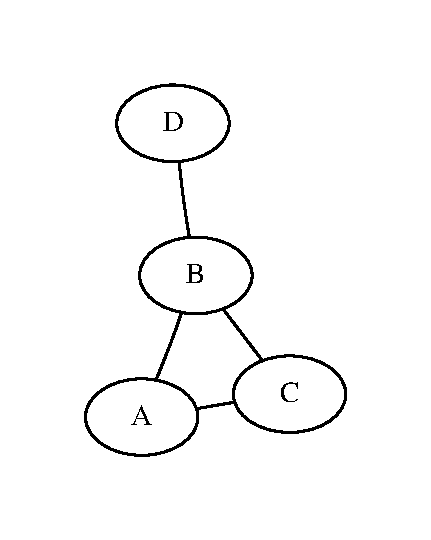
\includegraphics[trim = .4in .4in .4in .4in, clip, height=1.15in]{7_sampleABC.pdf}} &&&&&& \\
& A B & & \textbf{A} & \textbf{B} & \textbf{C} & \textbf{D} \\
& A C & \textbf{A} & 0 & 1 & 1 & 0\\
& B C & \textbf{B} & 1 & 0 & 1 & 1\\
& B D & \textbf{C} & 1 & 1 & 0 & 0\\
& & \textbf{D} & 0 & 1 & 0 & 0\\
&&&&&&\\
\hline
\end{tabular}
\caption{Three ways of representing the same network}
\end{center}
\end{figure}

\DefineShortVerb{\|}
The advantages of the graphic representation are obvious: our brains can very quickly process the lines and ovals.  
If we want a simple way to store it, however, we might use an edge list: using a minimum of formatting, we can create 
a very succinct file that completely describes the network structure.  Finally, the adjacency matrix allows us to efficiently 
work with the network algorithmically.  Both the edgelist and adjacency matrix models are easy to represent in Python as 2-dimensional 
data structures: a list of lists and a dictionary\footnote{A dictionary in Python is a type of variable similar to a list, except that 
indices can be any unique value, rather than strictly consecutive integers.  In this case, we would use the unique node names.} of 
dictionaries, respectively.  Working with multi-dimensional data structures is beyond the scope of this course\textemdash we will use NetworkX
instead\textemdash but I encourage you to learn about them if you continue working with Python.


\section{Diving into NetworkX}
\label{diving}
The NetworkX manual is over 200 pages long, but the developers have worked hard to keep simple things simple.  We'll go into more detail later,
but for now, let's start with an example.  Consider the following small network:

\begin{figure}[h]
\label{toy_net}
\begin{center}
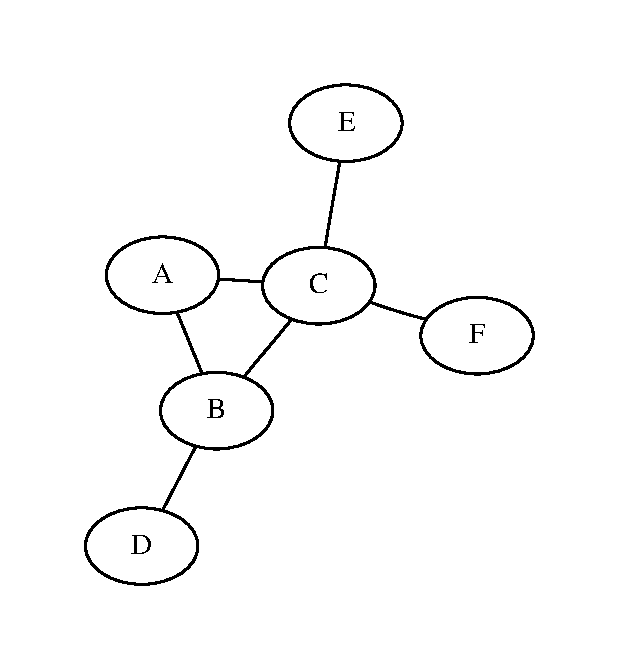
\includegraphics[trim = .4in .4in .4in .4in, clip, width=2.5in, height=2.5in]{7_sampleA-F.pdf}
\caption{Toy network}
\end{center}
\end{figure}

Let's reconstruct this toy network.  Open up IDLE/IPython, and begin typing the following lines (ignore any warnings about the ``sets module'', and you can leave off the comments, of course):

\begin{Verbatim}[samepage=true]
>>> from networkx import *       # import ALL of the functions available in NetworkX
>>> G = Graph()                  # Create a new, empty graph called G
>>> G.add_edge('A', 'B')         # Add an edge from node 'A' to node 'B'
>>> G.add_edge('A', 'C')         # Adding edges automatically creates the nodes
>>> G.add_node('E')              # We can also explicitly create nodes
>>> G.add_edge('E', 'C')         # And THEN connect them
>>> # Continue adding the other three edges in the toy network diagram
\end{Verbatim}

When you think you have all of the edges added, take a look at your network by entering the code below.  Just like in the exercise at the end of the last lab, you may need to use the |show()| function in the |pylab| library to handle opening a new window on the screen.

\begin{Verbatim}[samepage=true]
>>> from pylab import show       # import show() from pylab
>>> draw(G)                      # Tell NetworkX to decide how to visualize the graph
>>> show()                       # Open a new window to display the output
\end{Verbatim}

If you find that the figure is drawn when you execute |draw(G)|, then you do not need to import or execute |show()|.  This unfortunately is system-specific. Also note that before you draw the network again, you may need to close the old window.

How does your graph look?  It won't be visually identical to Fig.~\ref{toy_net}, but does it have all of the right nodes 
and edges? In case you want to remove parts of the network, you can do so with the following functions:

\begin{Verbatim}[samepage=true]
>>> G.remove_edge('A', 'C')      # Delete the edge between 'A' and 'C' (won't delete nodes)
>>> G.remove_node('A')           # Delete 'A' from the network, along with all its edges
\end{Verbatim}
\pagebreak
What if your network is getting really large, or you need a programmatic way to check whether the network structure is right?  
Try each of these functions:

\begin{Verbatim}[samepage=true]
>>> G.nodes()                    # Get a list of all nodes
>>> G.edges()                    # Get a list of all edges
>>> G.order()                    # Get the number of nodes
>>> G.size()                     # Get the number of edges
\end{Verbatim}

\section{Automating network construction}
Most of the time you will not want to be building and editing graphs by hand.  Open a new document in your text editor, and begin writing a program that will reproduce what you just did manually.  Here's a head start:

\begin{Verbatim}[numbers = left, samepage=true]
#!/usr/bin/python
from networkx import *
from pylab import show

G = Graph()

#
# insert code here to add all of the "toy network" edges
#

draw(G)
show()
\end{Verbatim}

Now you can run your program by pressing |CONTROL-r| or by going to Run\textgreater Run File.  If your program doesn't work and you get error
 messages, usually it's the last error message that you want to focus on.  If you're stuck, let me know and I'll come help.

\section{Constructing a network from an edgelist file}
\label{edges_to_net}
The last exercise was an important step forward: by putting all of the code in one file instead of using IDLE, we have a better record of exactly what
we did, we can easily change steps as necessary, and we can run it whenever we need to.  Still, typing one line of code for every edge in the network
does not scale well at all, and it's not a generic solution.  It would be better to read in an arbitrary edge list file and create the network from that.
I'll provide you with the |toy_edges.csv| file.

Start writing a new program, again using the ``head start'' code from the last example.  This time, however, replace the three commented lines with 
code that

\begin{itemize}
\item opens the |toy_edges.csv| file
\item loops through each line in the file
\item splits the line into the two node names\textemdash remember to split on commas instead of spaces!
\item adds an edge to the network connecting those two nodes
\end{itemize}

If you're having a hard time remembering how to do that in Python (that's okay!), take a look at the code from Lab 2, Section 7: Determining degree
 sequence and distribution.  As always, let me know if you get stuck.  When you're done, run your program and check the results!

\pagebreak

\section{Analyze a sexual contact network with NetworkX}

\UndefineShortVerb{\|}
\begin{figure}[!ht]

\begin{center}
\begin{tabular}{cc}
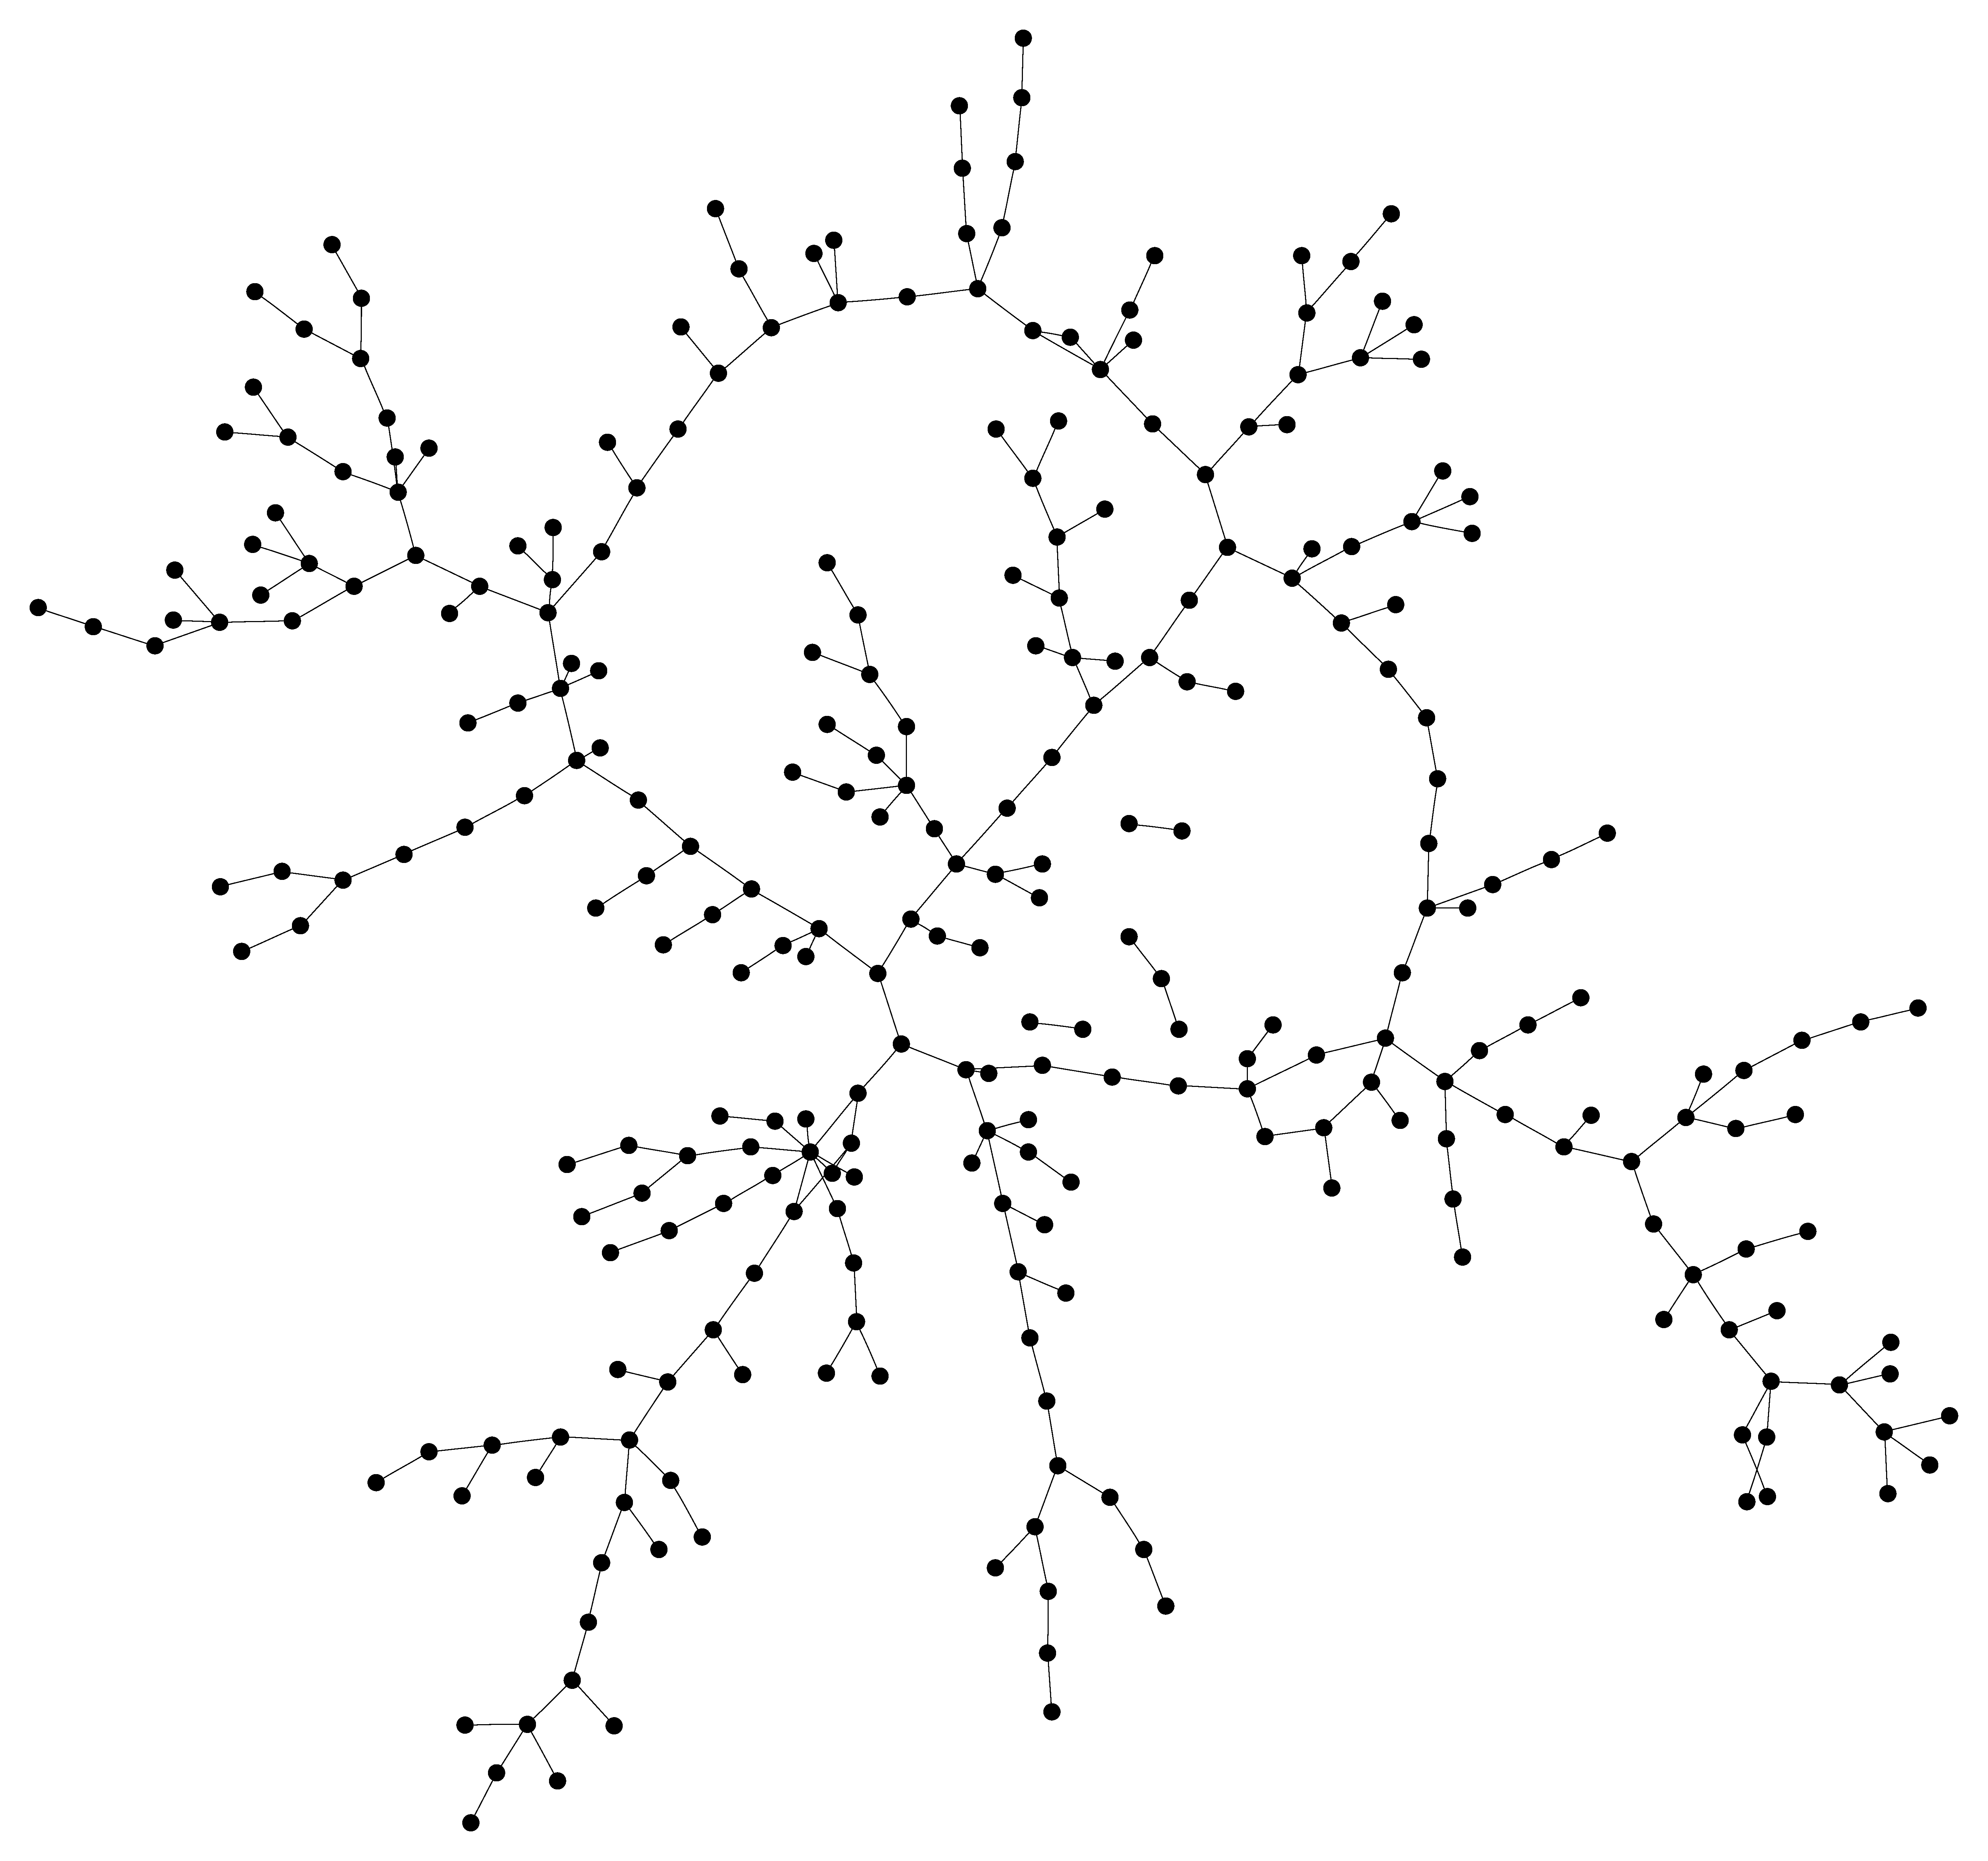
\includegraphics[width = 3in]{sexual_net.pdf} &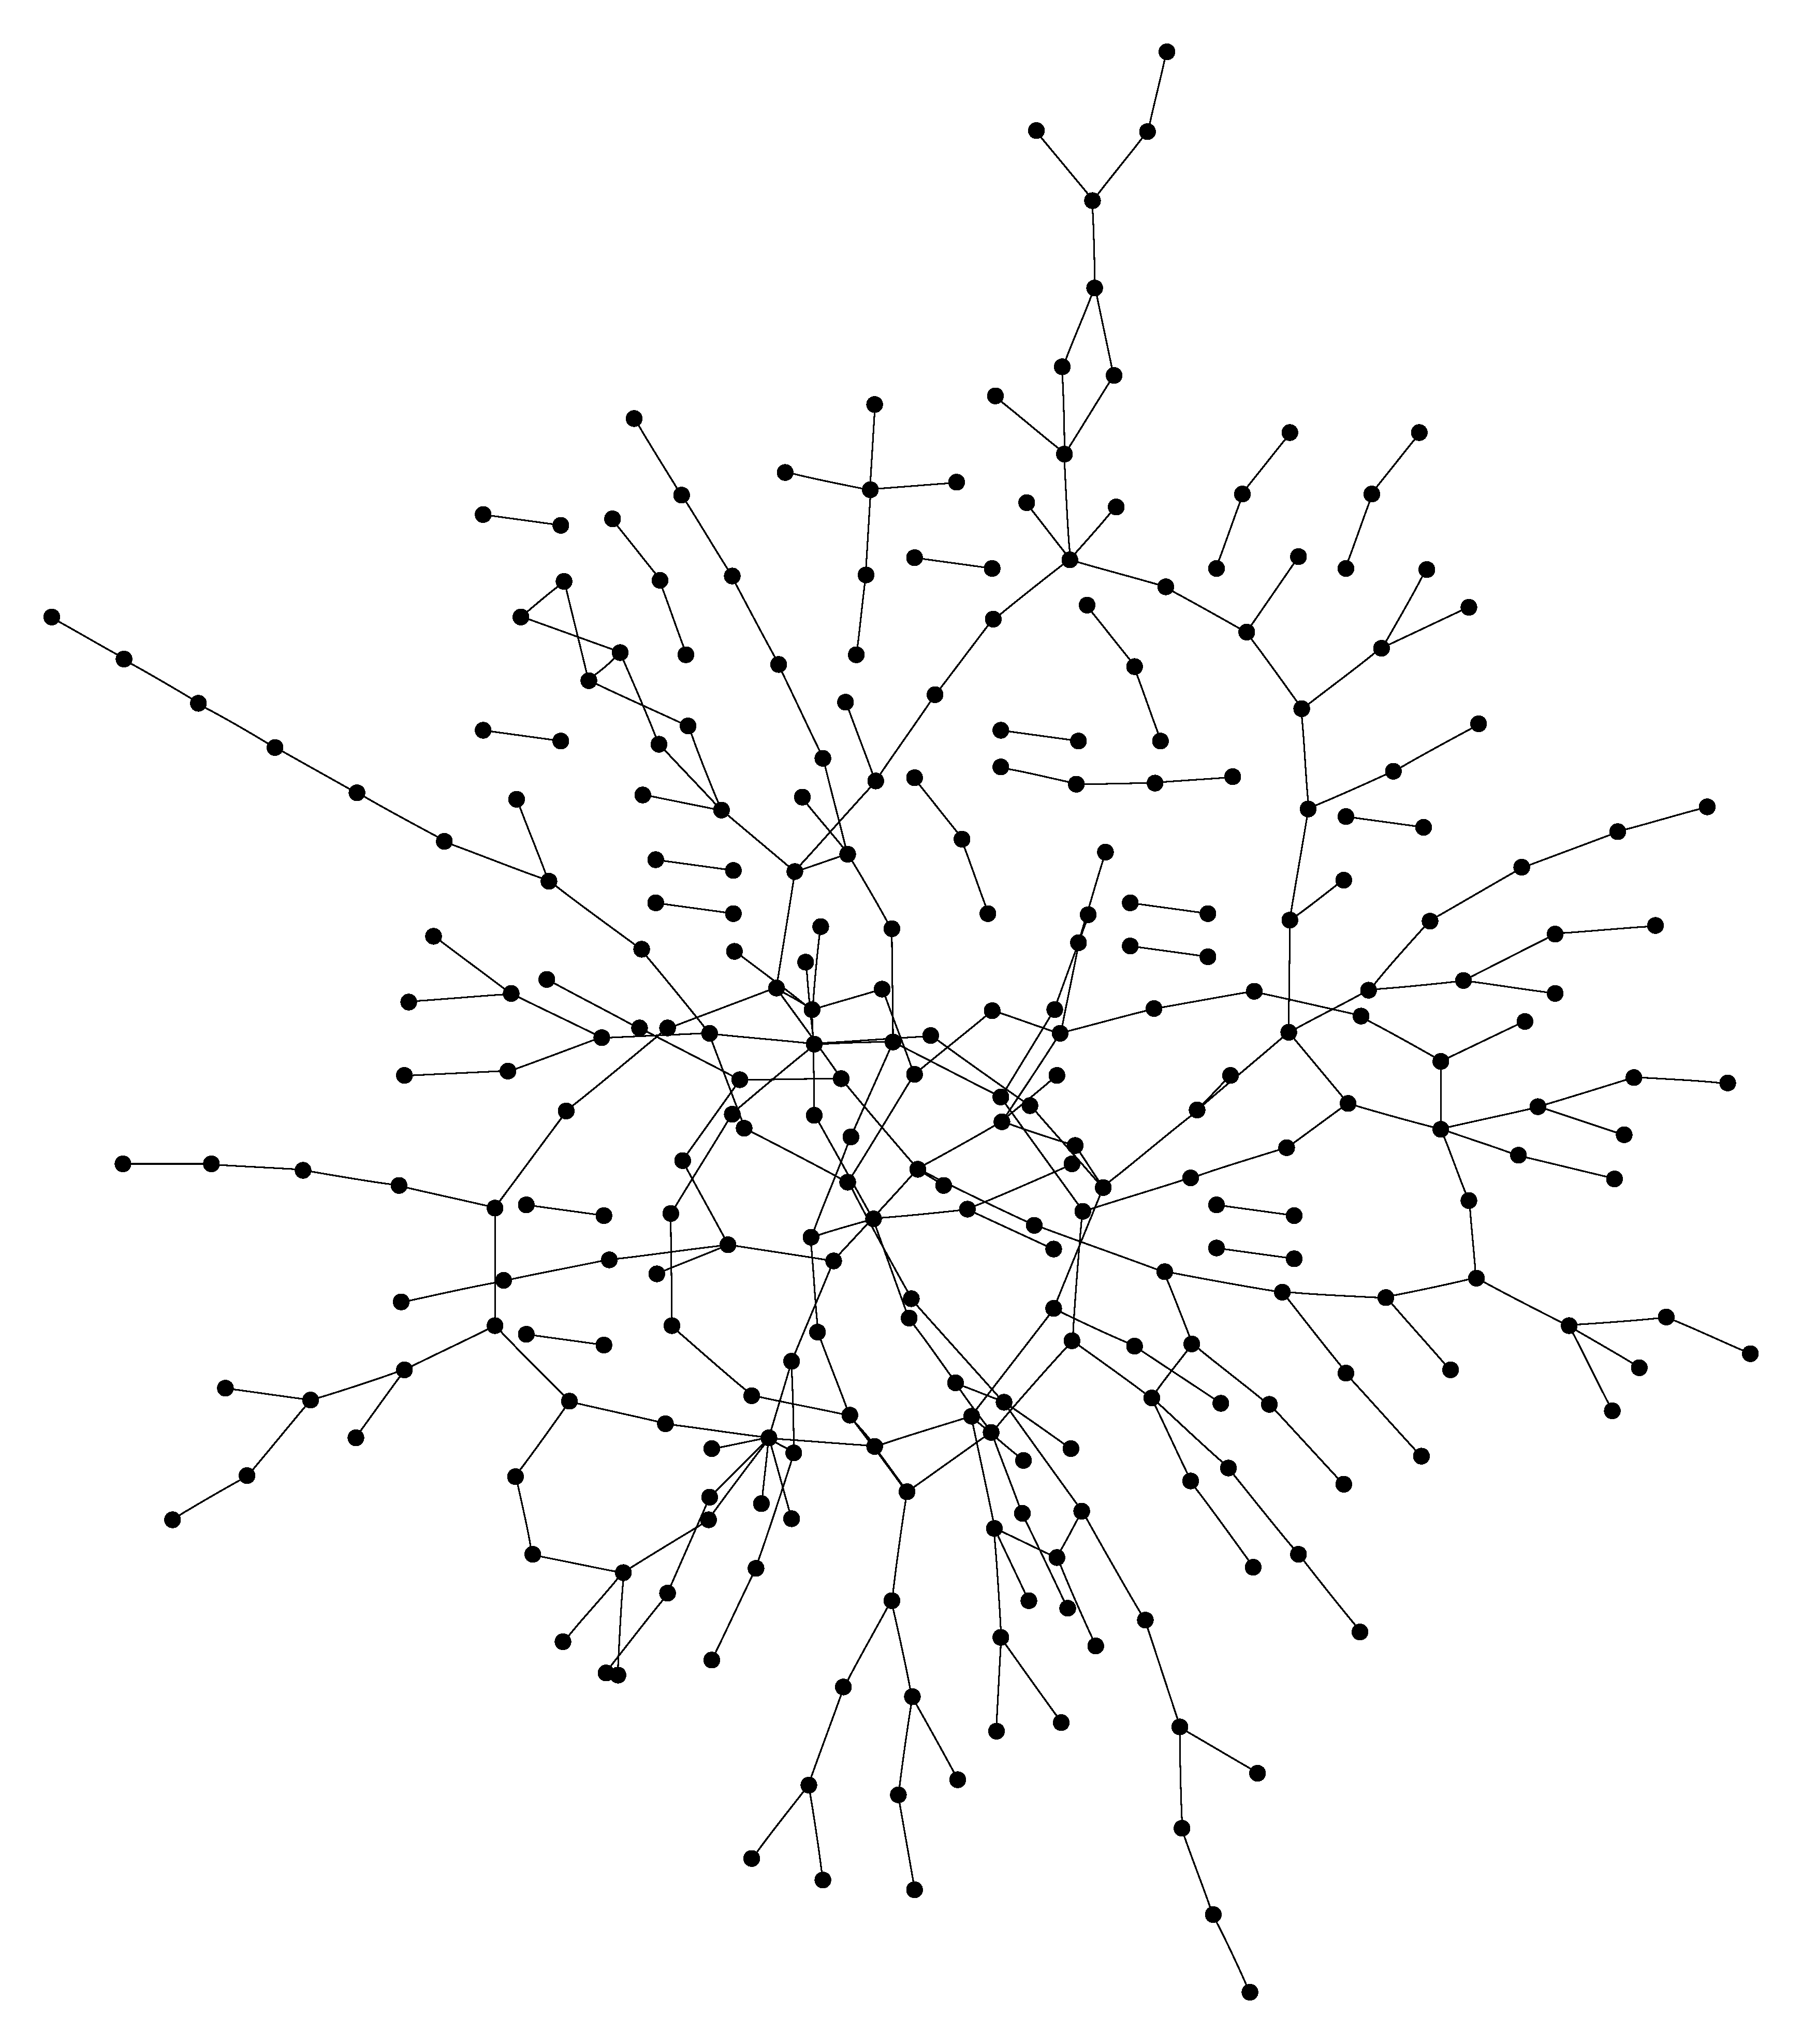
\includegraphics[width = 3in]{shuffled_sex.pdf}\\
\textbf{(a) Real sexual network} & \textbf{(b) Randomized sexual network}\\
\end{tabular}
\caption{Comparison between actual and randomly connected network (same degree sequence)}
\label{sex_fig}
\end{center}
\end{figure}
\DefineShortVerb{\|}

The network of sexual contacts\footnote{based on data from Bearman, P., J. Moody and K. Stovel. ``Chains of Affection: The 
Structure of Adolescent Romantic and Sexual Networks.'' American Journal of Sociology. 110:44-91, 2004.} depicted in Figure~\ref{sex_fig}a is based on the real interactions of a 
group of adolescents in a town in the midwestern United States over a period of 18 months.  As described by the authors of the study, the network is
``characterized by long contact chains and few cycles.''  So that you have a basis for comparison, if we keep the number of nodes and their degrees the same,
but we thoroughly shuffled the connections between them, we get a graph that looks more like the one in Figure~\ref{sex_fig}b.

For now, we will work with the real network.  It is small enough that we can see some 
interesting structure, but big enough that we wouldn't want to calculate properties like mean degree by hand. 
 Using the file |sexual_net.csv| and the program you wrote in Section~\ref{edges_to_net}, you can already reconstruct this network 
in NetworkX (although it's a bit too large to draw using NetworkX).

Here are some additional functions that you will likely find useful in this exercise:
\begin{Verbatim}[samepage=true]
min(number_list)                # minimum value in the list
max(number_list)                # maximum value in the list
sum(number_list)                # sum values in the list
G.degree().values()             # the degree sequence (a list; use this to make histograms)
G.degree(52)                    # the degree of node 52
G.degree()                      # a labeled degree sequence (dicitonary of id, degree pairs)
number_connected_components(G)  # the number of disjoint subgraphs
\end{Verbatim}

Start with the code from your program from Section~\ref{edges_to_net}, but delete the |draw(G)| and |show()| lines.  You might want to re-save your 
program at this point as a different file.

Using the NetworkX functions supplemented with your own code, answer the following questions:
\begin{itemize}
 \item How many nodes and edges does the network have?
 \item What is the highest, lowest, and mean degree in the network?
 \item How many components are there?  (FYI, Figure~\ref{sex_fig}b has 21)
 \item Look at the degree distribution (i.e. create a histogram of the degree sequence).  How would you describe it?  How many modes (peaks) 
does it have, and where are they?  Does it look like any distributions you are familiar with?
\end{itemize}

Just to reiterate, the answers to the above questions are the same for both graphs in Figure~\ref{sex_fig}, except for the number of components.

\section{Analyze the semi-empirical Vancouver network}
Let's take a step up in scale, since that's what makes these programmatic solutions 
really worthwhile. We will be using a semi-empirical urban network\footnote{based on data from Meyers, L., B. Pourbohloul,
 M. Newman, D. Skowronski and R. Brunham. ``Network theory and SARS: predicting outbreak diversity.'' Journal of Theoretical Biology. 2004.},
developed in response to the 2003 SARS outbreak and based largely on census data for
Vancouver, Canada.  While we will refer to the network data used in this section
as ``the urban network,'' you should keep in mind that this is still a generated
network, and there are an infinite number of other such networks that could be
generated to have similar properties.  In our case, the network represents the
people living in 1,000 households; the edge list file is |urban_net.csv|.

Answer the same questions as before for this network:
\begin{itemize}
 \item How many nodes and edges does the network have?
 \item What is the highest, lowest, and mean degree in the network?
 \item How many components are there?
 \item How would you describe the degree distribution for the urban network?
\end{itemize}

In terms of how an infectious disease would propagate through the networks, what do you think are some important differences between 
the urban network and the sexual network? If we took the same individuals in the sexual contact network, but instead connected them based 
on their ``respiratory contacts,'' how would that network look different?

\section*{Additional exercise}
Make your program more generic, so that it prompts the user for an edge list filename, and then prints out nicely formatted descriptive statistics for
the network.  In order to get the filename from the user, use the function |raw_input()| instead of |input()|\textemdash the difference is that
|raw_input()| expects a text string, whereas |input()| requires numerical values or quoted strings.


\end{document}
